\section{Architectural Views}

\subsection{Context View}

\subsubsection{Stakeholders' Uses of This View}

\subsubsection{Context Diagram}

% Checked in grammarly
\afetbilgi \cite{afetbilgi} is not part of a more extensive system. It is a standalone and open-source efforted website to verify critical information in the fight against the 6 February 2023 Pazarcik Earthquake and deliver it to disaster victims and those who want to help in an understandable, concise manner in multiple languages.

This information is presented in either the form of legible tables with third-party governmental and private links or an interactable method via a map view interface. If deemed necessary, admin and maintainers can make changes to display newly created or edited data and upload it to the system upon any complaints or suggestions they may get on their contact details.

\begin{figure}[H]
  \centering
  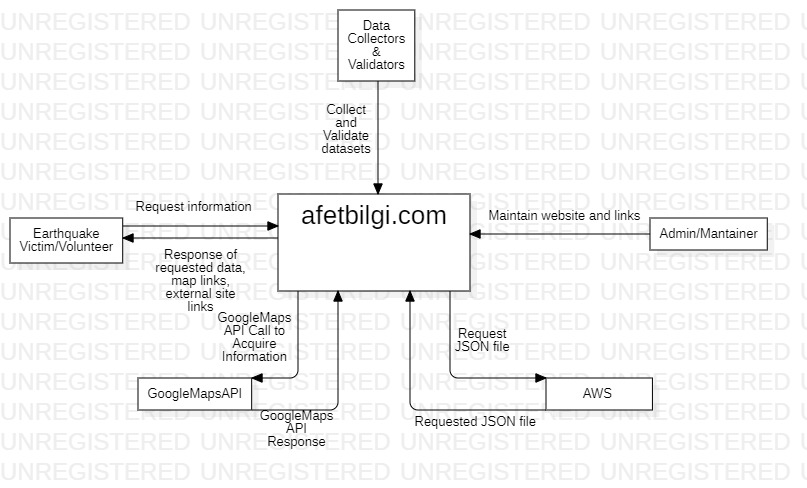
\includegraphics[width=\linewidth]{img/context-diagram.jpg}
  \caption{Context Diagram for \afetbilgi}
\end{figure}

The \afetbilgi\ consists of a combination of small physical and software parts. With the help of interfaces, these parts communicate among themselves and with the user.

\subsubsection{External Interfaces}

\begin{figure}[H]
  \centering
  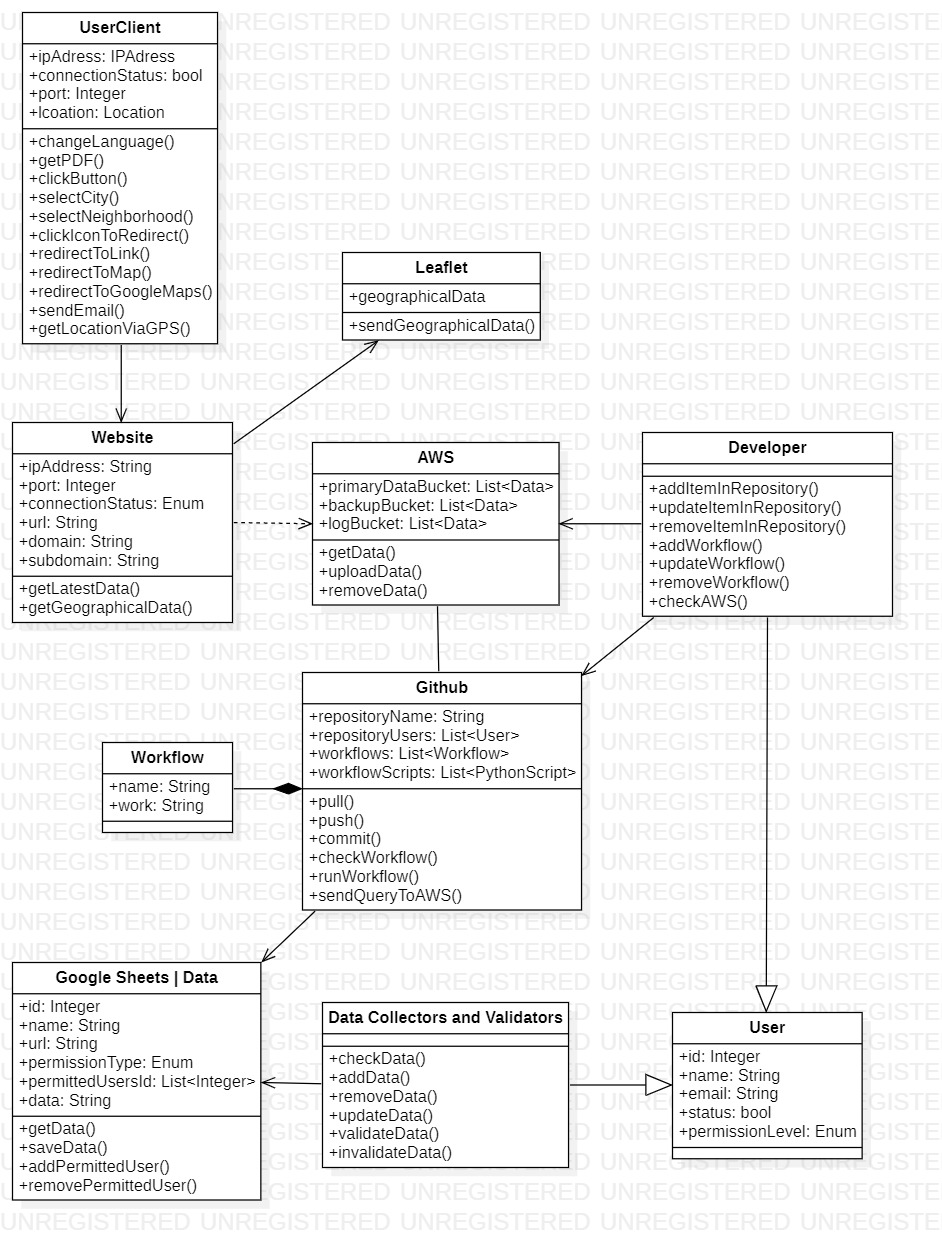
\includegraphics[width=\linewidth]{img/external-interfaces-diagram.jpg}
  \caption{External Interfaces}
\end{figure}

\subsubsection{Interaction Scenarios}

\begin{figure}[H]
  \centering
  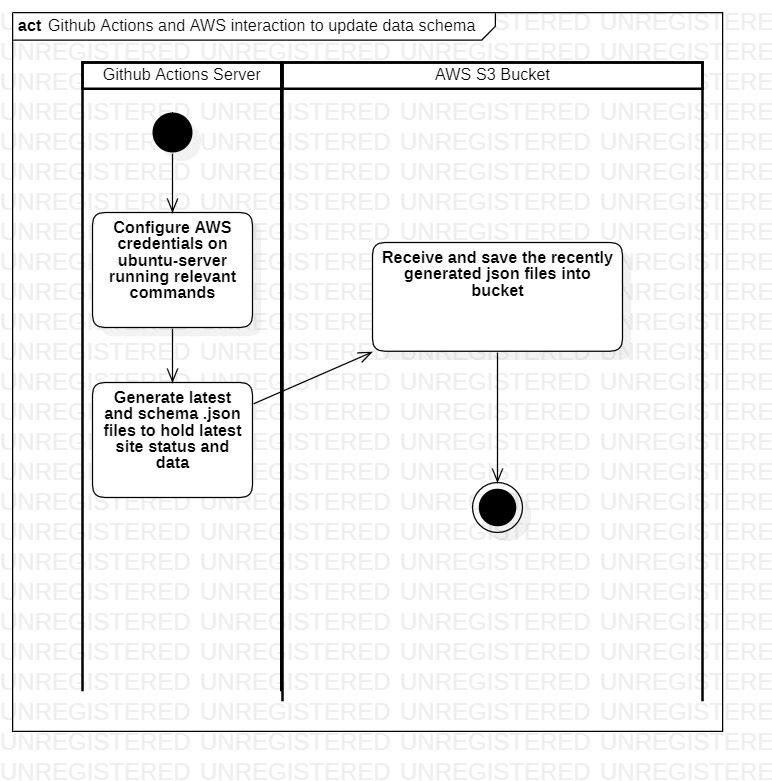
\includegraphics[width=\linewidth]{img/activity-diagram-1.jpg}
  \caption{Activity Diagram | GitHub Actions and AWS Interaction to Update Data Schema}
\end{figure}

\begin{figure}[H]
  \centering
  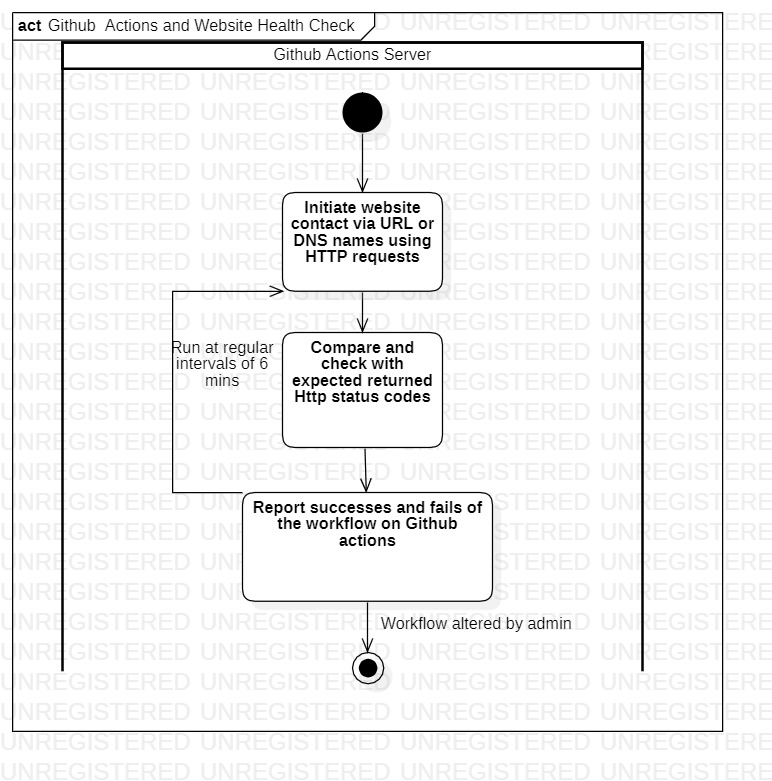
\includegraphics[width=\linewidth]{img/activity-diagram-2.jpg}
  \caption{Activity Diagram | GitHub Actions and Website Health Check}
\end{figure}

\subsection{Functional View}

\subsubsection{Stakeholders' Uses of This View}

\subsubsection{Component Diagram}

\begin{figure}[H]
  \centering
  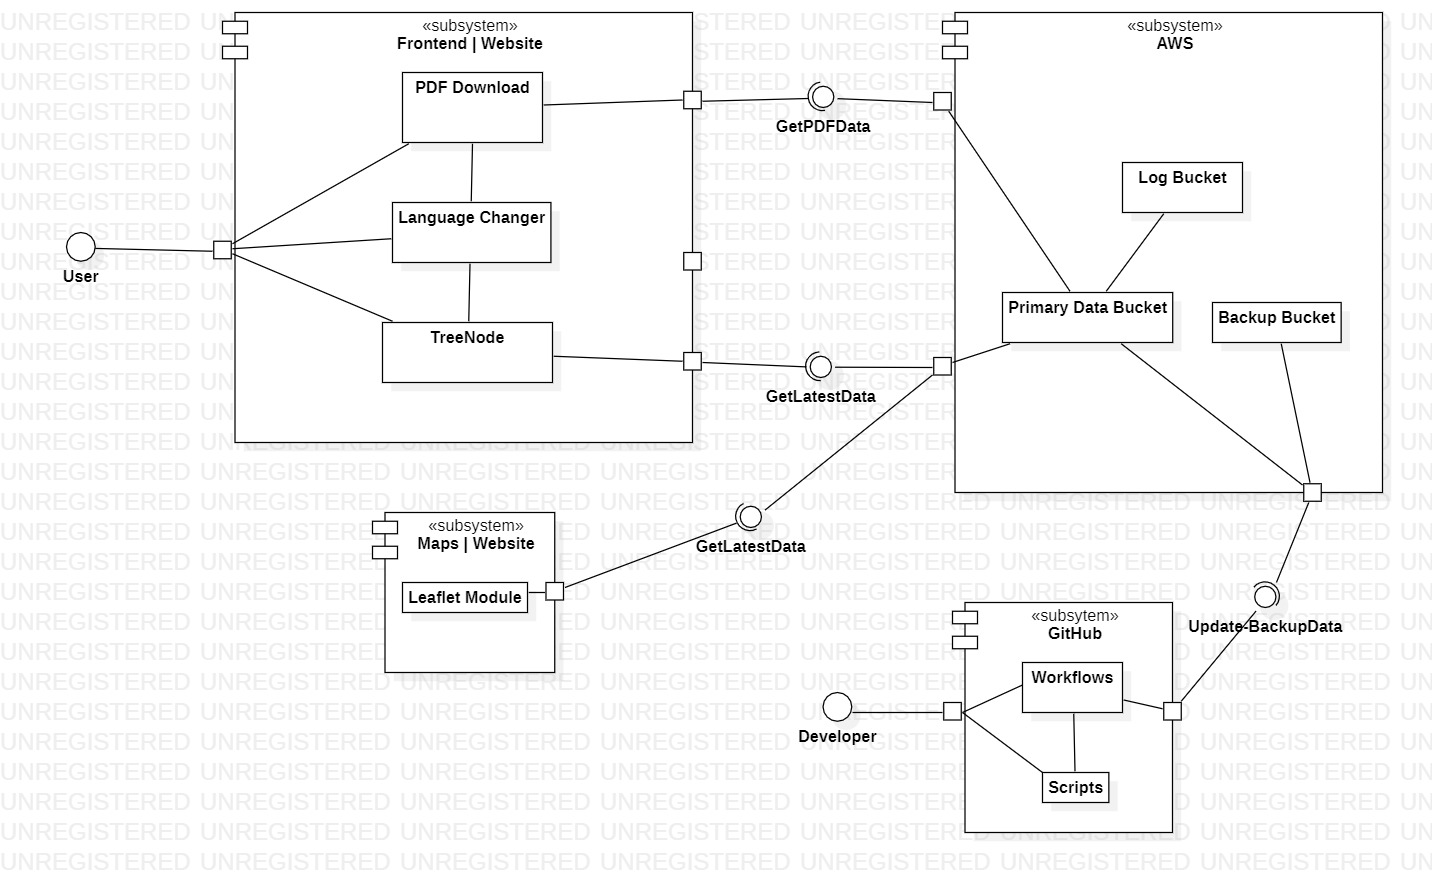
\includegraphics[width=\linewidth]{img/component-diagram.jpg}
  \caption{Component Diagram}
\end{figure}

\subsubsection{Internal Interfaces}

\begin{figure}[H]
  \centering
  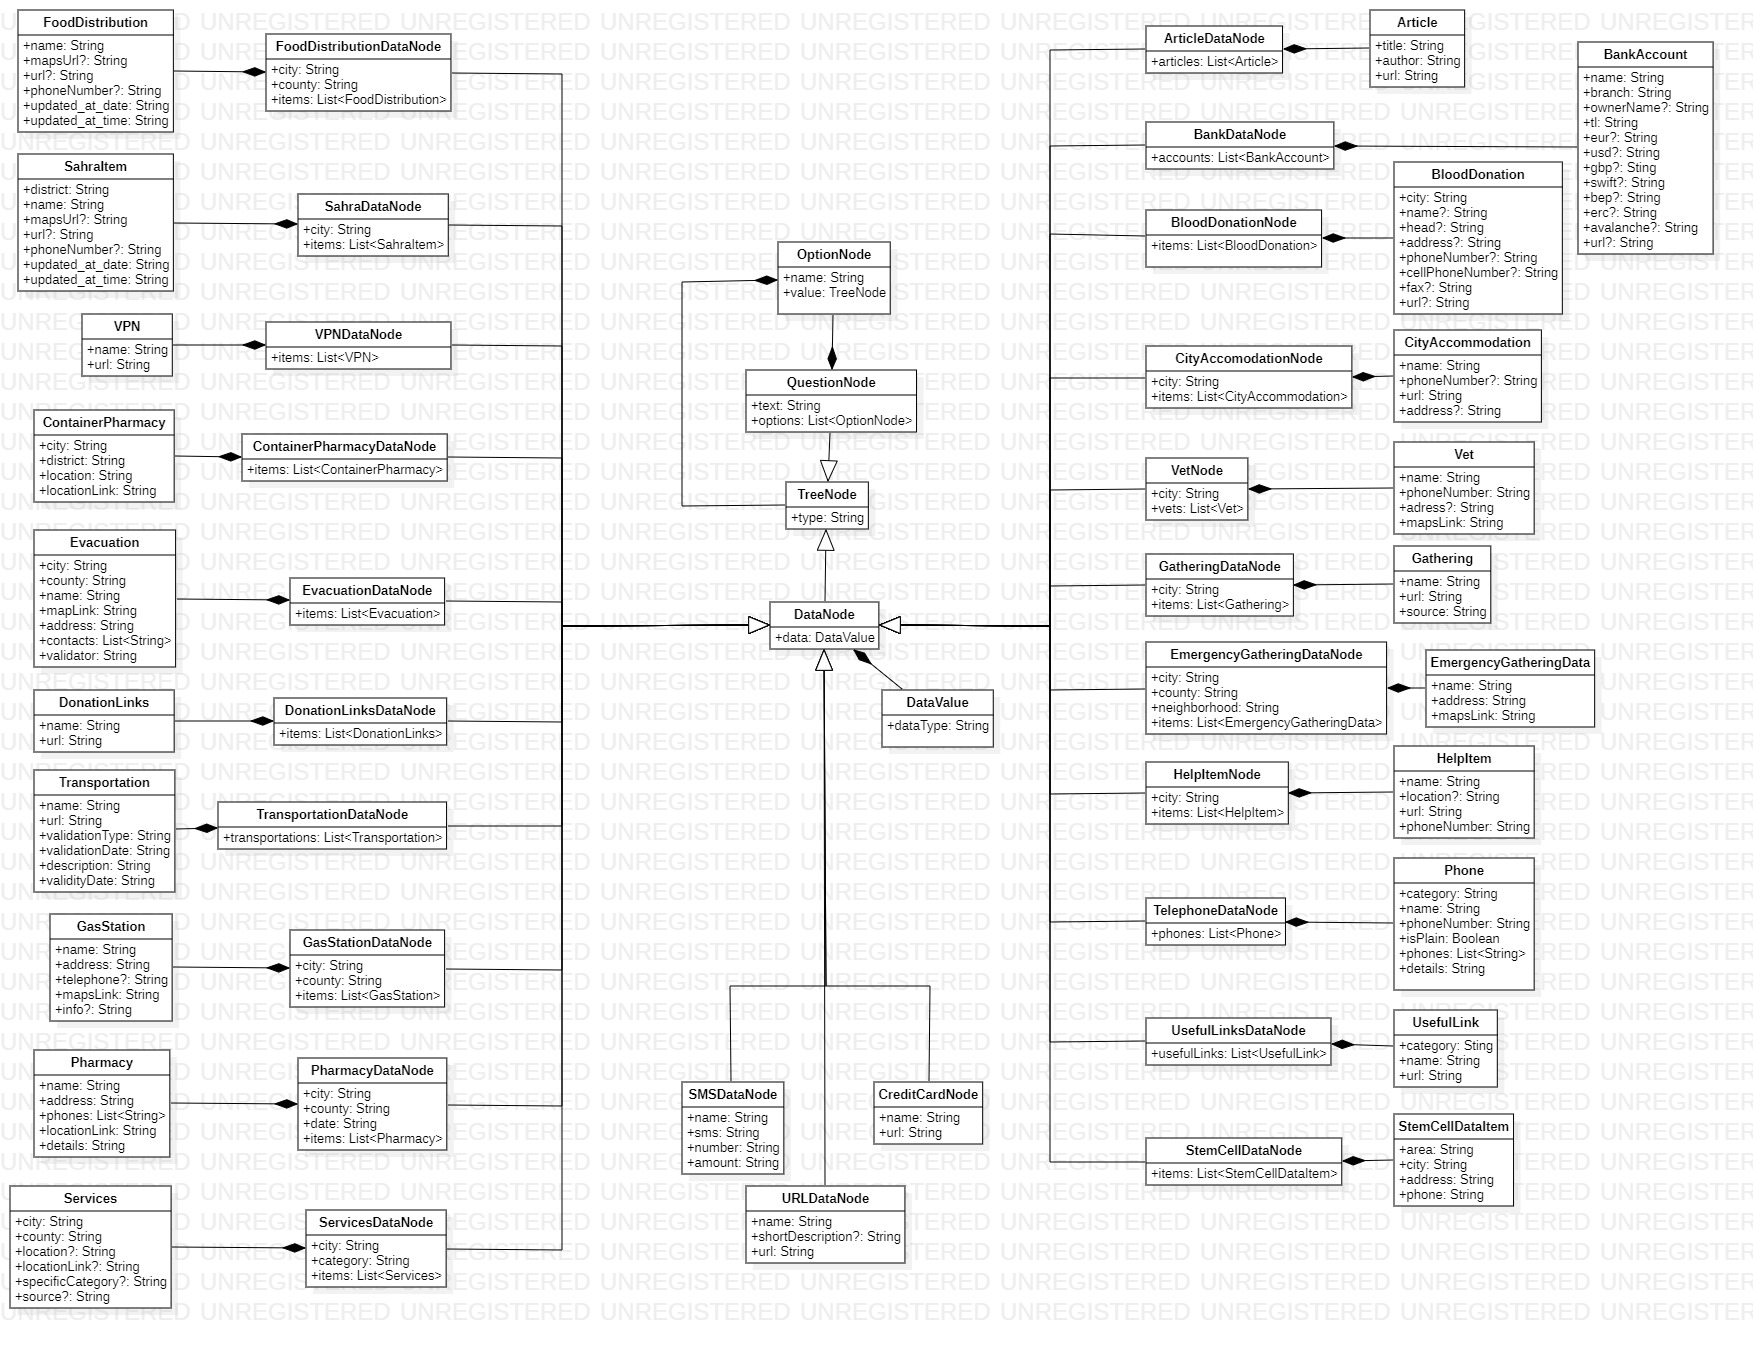
\includegraphics[width=\linewidth]{img/internal-interfaces-diagram.jpg}
  \caption{Internal Interfaces}
\end{figure}

\subsubsection{Interaction Patterns}

\begin{figure}[H]
  \centering
  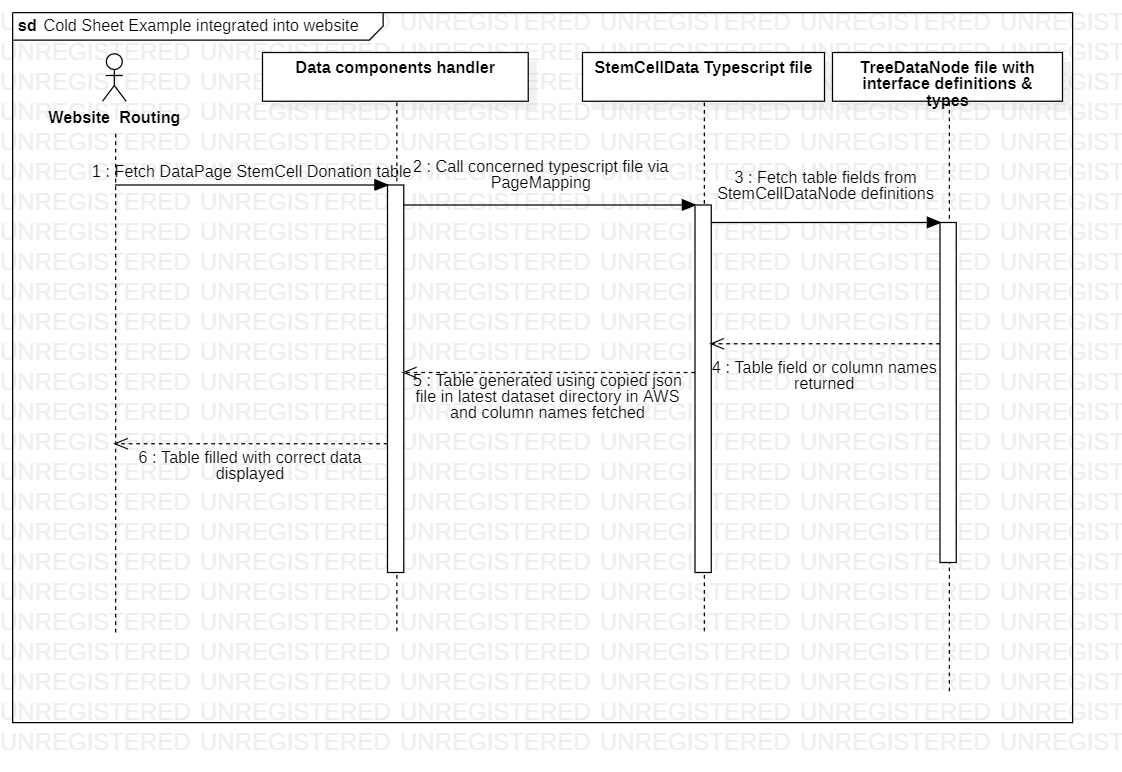
\includegraphics[width=\linewidth]{img/sequence-diagram-1.jpg}
  \caption{Sequence Diagram | Cold Sheet Example Integrated Into Website}
\end{figure}

\begin{figure}[H]
  \centering
  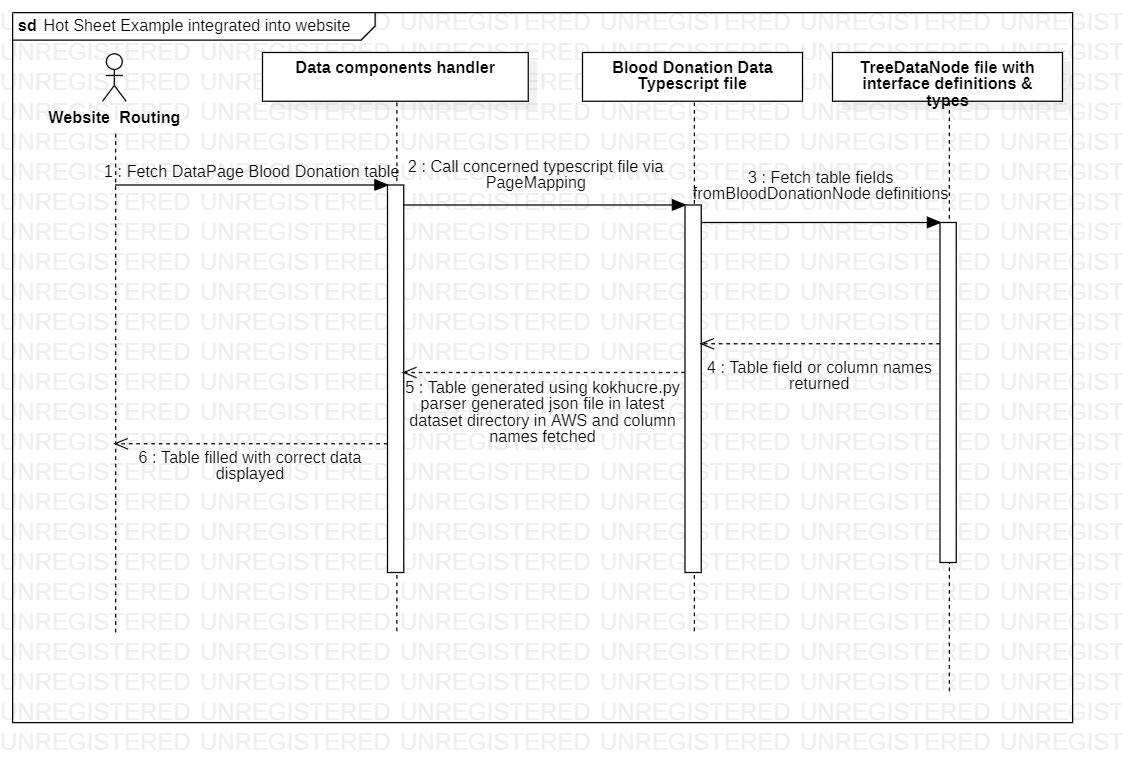
\includegraphics[width=\linewidth]{img/sequence-diagram-2.jpg}
  \caption{Sequence Diagram | Hot Sheet Example Integrated Into Website}
\end{figure}

\begin{figure}[H]
  \centering
  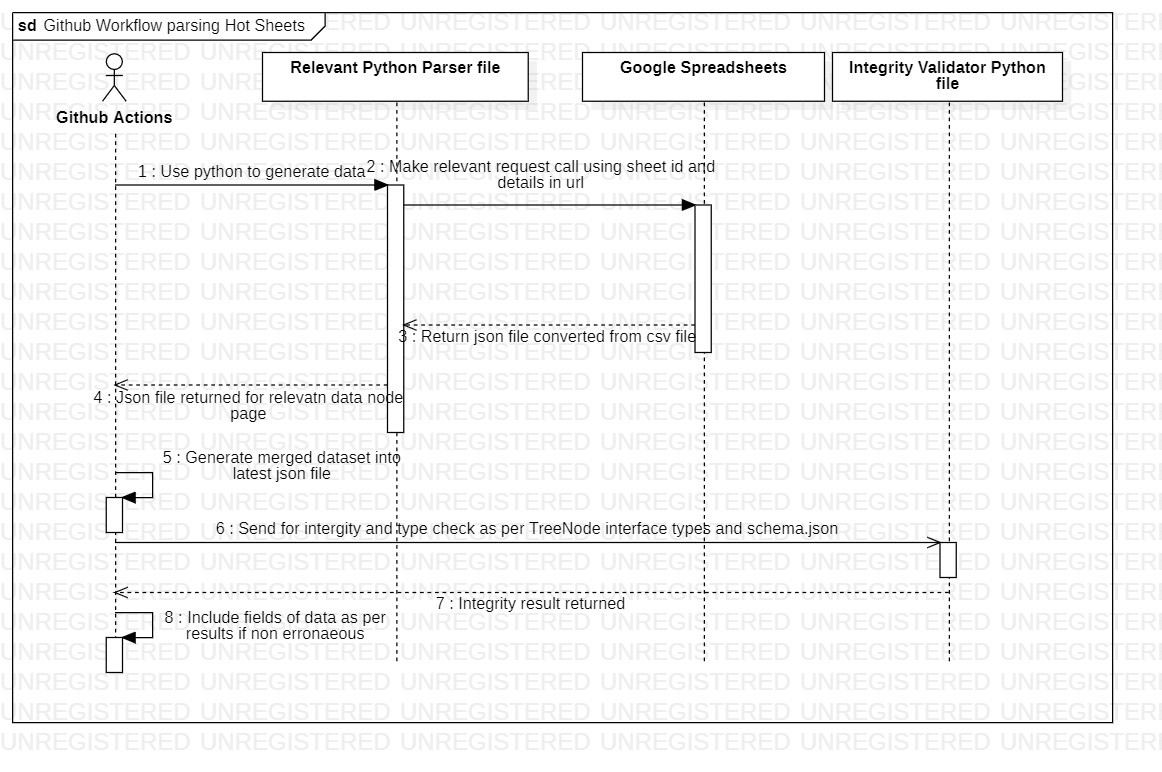
\includegraphics[width=\linewidth]{img/sequence-diagram-3.jpg}
  \caption{Sequence Diagram | GitHub Workflow Parsing Hot Sheets}
\end{figure}

\subsection{Information View}

\subsubsection{Stakeholders' Uses of This View}

\subsubsection{Database Class Diagram}

\begin{figure}[H]
  \centering
  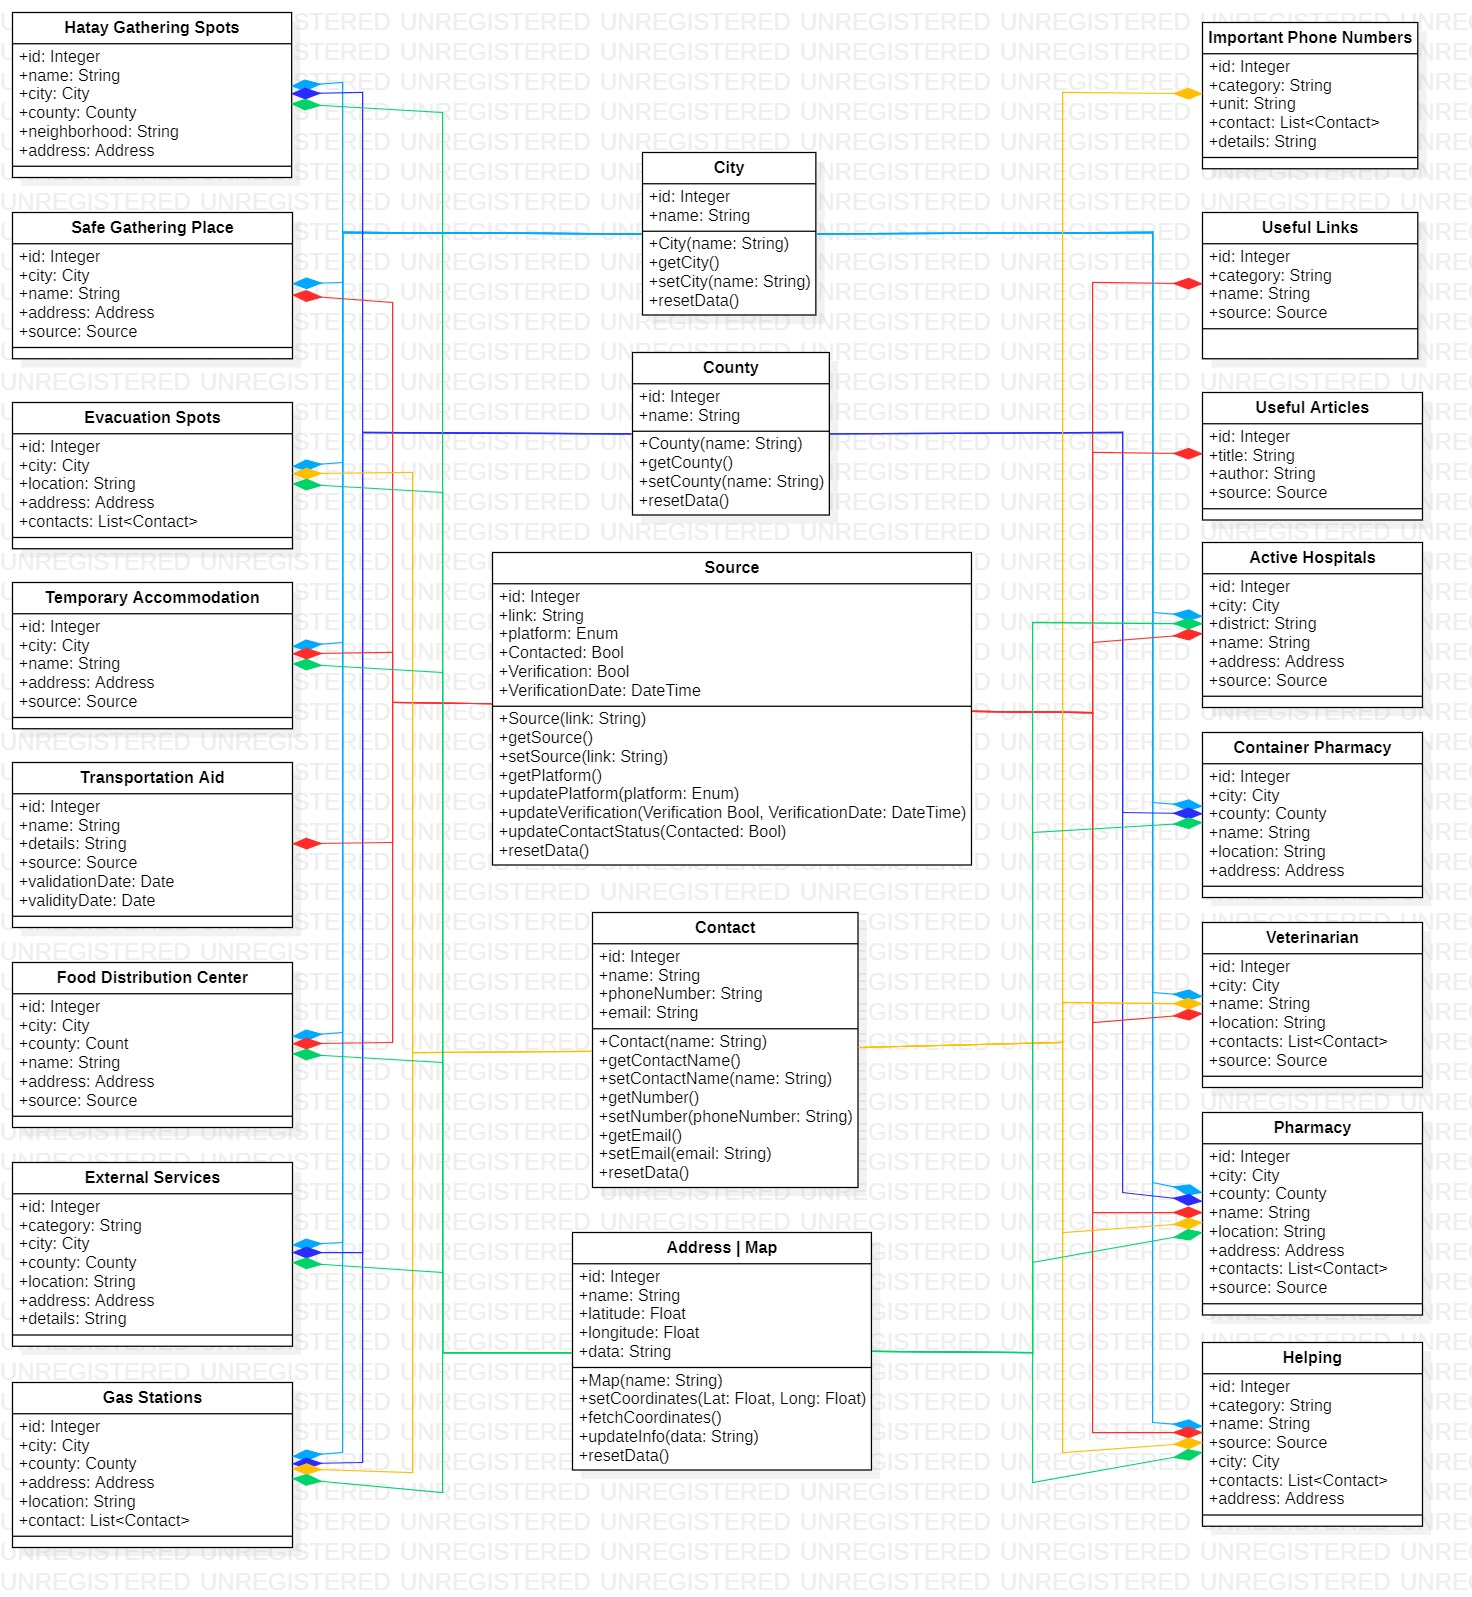
\includegraphics[width=\linewidth]{img/database-class-diagram.jpg}
  \caption{Database Class Diagram}
\end{figure}

\subsubsection{Operations on Data}

\subsection{Deployment View}

\subsubsection{Stakeholders' Uses of This View}

\subsubsection{Deployment Diagram}

\begin{figure}[H]
  \centering
  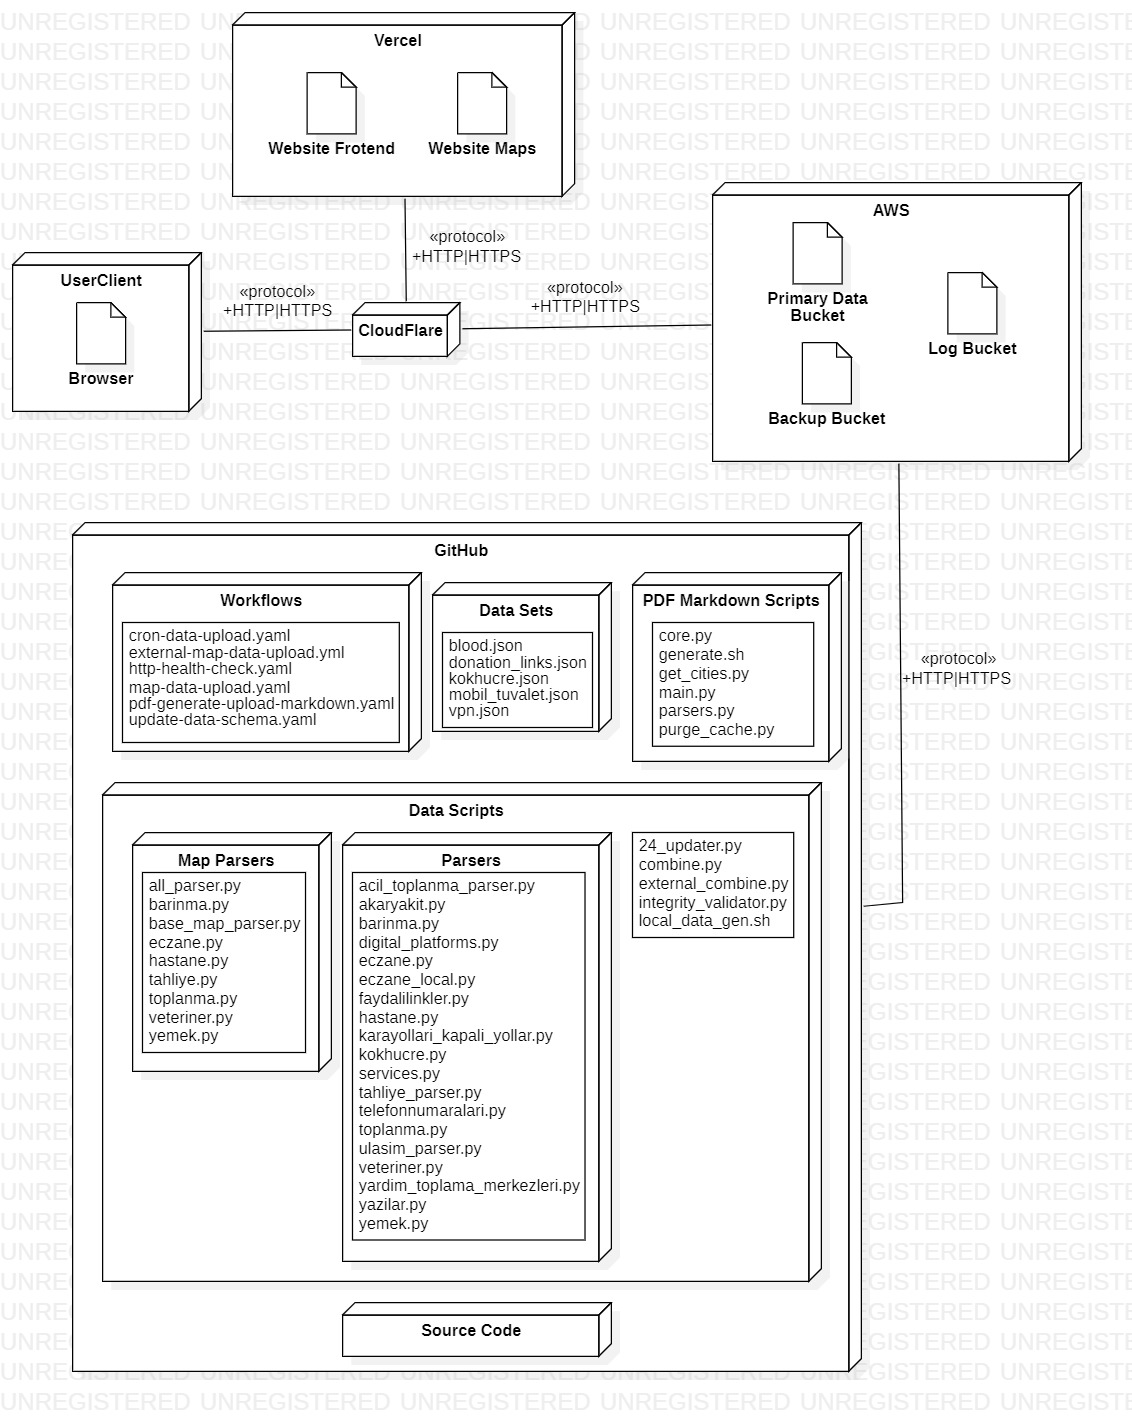
\includegraphics[width=\linewidth]{img/deployment-diagram.jpg}
  \caption{Deployment Diagram}
\end{figure}

\subsection{Design Rationale}
